\section{Discrete phase transitions}

During the whole course we have mainly focus on the description of physical systems behaves inside a particular phase, allowing us to understand which phase is stable at certain conditions. Nevertheless, another important question that we want to answer is how the transition to one phase to another happens exactly. We have talked, when we faced phase diagrams, how certain materials are able to go from one state to another in particular situation in a qualitative way, here we aim in describing it mathematically using the tools obtained from equilibrium Thermodynamics and kinetics.

The first thing that we shall say is that a phase transformation happens when, due to variation of certain parameters such as temperature or external field, the system breaks some internal symmetry finding more advantages to restructure itself in a more or less ordered way. For this reason, we are going to describe such phenomena using a set of parameters $\xi$ that mainly describes the order that is present inside the material, called \textbf{order parameters}. We have already seen some example of them in previous studies: like the long range order $\eta$ and the fractional density $X_i$ inside the study of the equilibrium inside a binary system. On a more general ground, during the study we will have to work with two main type of order parameters that we need to take into account, and we will define as follows.
\dfn{Conserved and Non-Conserved order parameters}
{
    An order parameter $\xi$ inside a system is conserved if it needs to be a constant inside a closed system, while non-conserved ones can change also if the system is closed.
}
\noindent
It's easy to understand that in the examples we have already seen $X_i$ is conserved, while $\eta$ is not. These two types of parameters highly influences how the transition behaves since the free energy will depend on them, $G(\xi)$, and based on their variation the energy landscape will be modified. To be more precise, we can evaluate a general form for the variation of free energy inside a material due to order parameters' changes in the two cases.
\thm{Variation for non-conserved $\xi$}
{
    Suppose that in a closed system composed of $N$ moles of material $n$ moles undergo a variation of a non-conserved order parameter from $\xi_1$ to $\xi_2$, where we assume $N\ll n$. The corresponding change of free energy of the whole system is
    \begin{equation}
        \delta G_u = n[G(\xi_2) - G(\xi_1)] \approx n G'(\xi_1)\delta\xi,
    \end{equation}
    where $G$ is the molar free energy of the material.
}
\pf{Proof}
{
    The proof is really simple since the order parameter is non-conserved it can change as wants inside the closed system, and so we can assume tha all the $N-n$ moles remains in $\xi_1$ being unperturbed by the change of the others. In this way we can set the change of free energy in the whole system as
    \begin{equation}
        \delta G_u = (N-n)G(\xi_1) + nG(\xi_2) - NG(\xi_1) = n[G(\xi_2) - G(\xi_1)].
    \end{equation}
    Also, the approximation with the first derivative is only the first order term of the Taylor series setting $\delta\xi \equiv \xi_2 - \xi_1$. 
}
\noindent
This shows how for non-conserved parameters the change totally relies only on the form of $G$ itself, with a behavior that is totally analogous to the one of the normal system. In the case of conserved parameters the thing changes a little becoming more interesting.
\thm{Variation for conserved $\xi$}
{
    Suppose that in a closed system composed of $N$ moles of material $n$ moles undergo a variation of a conserved order parameter from $\xi_1$ to $\xi_2$, where we assume $N\ll n$. The corresponding change of free energy of the whole system is
    \begin{equation}
        \label{eq:ConservedChange}
        \delta G_c = n\{G(\xi_2) - [G(\xi_1) + G'(\xi_1)(\xi_2 - \xi_1)]\} \approx \frac{n}{2} G''(\xi_1)\delta\xi^2,
    \end{equation}
    where $G$ is the molar free energy of the material.
}
\pf{Proof}
{
    In this case the total order parameter inside the material could not change, still $\xi$ can have local variation that can be compensated by the variation of the order parameter of the rest of the material. Meaning that, if $n$ moles now have $\xi_2$ as order parameter then all the remaining $N-n$ one's needs to have $\xi_1 - \Delta$ to compensate as follows 
    \begin{equation}
        (N-n)(\xi_1 + \Delta) +n\xi_1 = N\xi_1,
    \end{equation}
    which gives $\Delta = n(\xi_1 - \xi_2)/(N-n)$ so that $N\Delta \approx n(\xi_1 - \xi_2)$. In this way we can write down the following variation
    \begin{equation}
        \delta G_c = (N-n)G(\xi_1 + \Delta) + nG(\xi_2) - NG(\xi_1) \approx (N-n)[G(\xi_1) + G'(\xi_1)\Delta] + nG(\xi_2) - NG(\xi_1),
    \end{equation}
    which gives exactly what we wanted. Then, to have the approximation we can write $\xi_2 = \xi_1 + \delta\xi$ and expand the value of $G(\xi_2)$ to the second order obtain the final result.
}
\noindent
\begin{figure}[t]
    \centering
    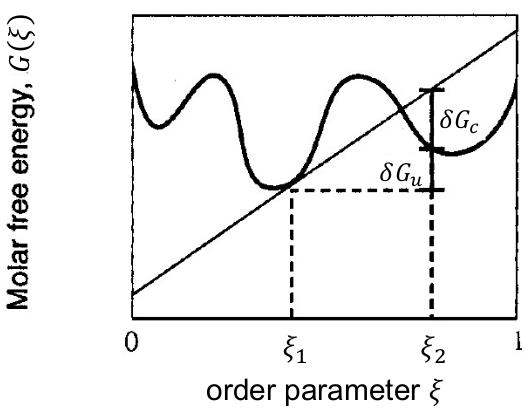
\includegraphics[width=0.4\textwidth]{Immagini/GVarXi.png}
    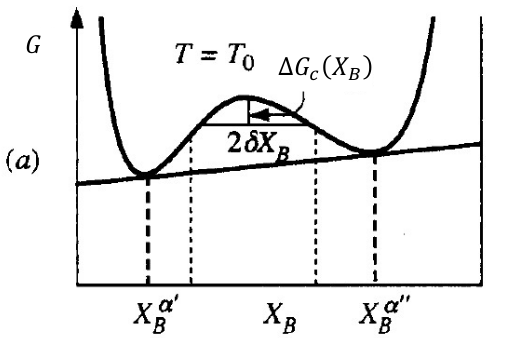
\includegraphics[width=0.45\textwidth]{Immagini/SpinodalPoints.png}
    \caption{
        Representation of a free energy landscape depending on order parameters with the opportune variations on the left, and a representation of a $G(X)$ with the spinodal points in evidence on the right.
    }
    \label{fig:FirstPhaseTrans}
\end{figure}
In this case the variation of the free energy do not simply depend on the form of $G$ but also on the convexity of it. In particular, the variation of free energy due to order changes is mainly given by the second derivative. Meaning that if we are in a local maximum $G'' < 0$ and the system is \textbf{unstable} wanting to change to a minimum where $G'' > 0$ so that even if $\xi$ changes the variation of energy is positive and the system is so \textbf{metastable}. Where we use the word metastable and not stable since it's not sad that the system will remain in that minimum forever, due to large variation of energy coming external factors, like thermal fluctuations, the system can jump to another valley and sit there for some time until another jump happens.

This description of how $G$ changes due to order parameters is really general and profound, showing us not only how the free energy changes based on the nature on the parameter itself, but also suggest to us how that change happens. Let's focus a moment on \eqref{eq:ConservedChange} in the situation depicted on \figref{fig:FirstPhaseTrans}, the system will have two metastable state divided by an energy barrier which defines an unstable region. In particular, the unstable region is delimited by the $\xi$ so that $G''(\xi) = 0$, where $X_B$ is the order parameter in that case. We have already talk about points with such a property calling them \textbf{spinodal points}, basically the region inside the spinodal points is unstable meaning that it will natural evolve continuously to a minimum. Then, when it reaches a metastable position it will sit there and remain there until a sudden discontinuous change happens, and the system changes minimum to sit in. These two different behaviors define the two main types of phase transitions that we are going to touch called \textbf{continuous} and \textbf{discontinuous} phase transitions, which mainly differ in how quick the change happens and in the extension of the change, having that discontinuous transformations are usually locals while continuous are more global. 

In this first section we will focus first on the discontinuous type describing the main, and simpler, possible forms of such transitions: like the formation of a water droplet in clouds. We will leave the continuous case to a further section.

\subsection{Nucleation theory}

Nucleation is an important phenomenon that consist in the spontaneous formation of cluster of components inside the material that will then grow over time through different mechanisms like coarsening. In particular, in the classical theory of nucleation the system goes through four different steps: an initial incubation where no cluster are formed over time, to then a steady-state situation where the number increase in time reaching a maxima where driving forces of nucleation start to reduce, and then the coarsening that will decrease the number generating bigger grains. Inside such a complex kinetic behavior we aim first in the description of the distribution of cluster inside cluster space $N_\nu(t)$, where $N_\nu$ is the number of cluster possessing $\nu$ monomers components inside them.

